\subsection{Интерференция в пленках и в пластинках}


\textbf{Тонкая плёнка}. 
Рассмотрим тонкую пленку толщины $d$ и показателя прелмления $n$. При освещении точечным истоником света, мы увилим разность хода лучей в 
\begin{equation*}
    \Delta = (A' C B') + \frac{\lambda}{2} = 2 n d \cos \psi + \frac{\lambda}{2},
\end{equation*}
где $\psi$ -- угол преломления, $\lambda/2$ -- следставие преломления от среды с большим показателем преломления. 
\begin{figure}[ht]
    \centering
    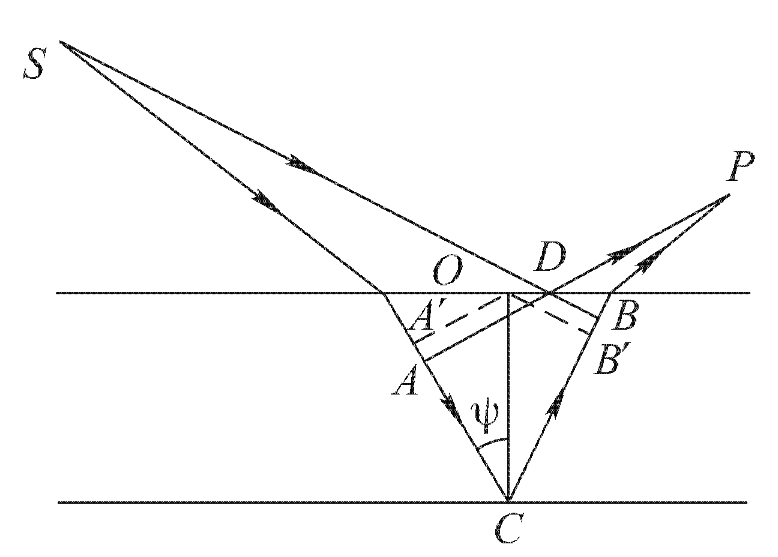
\includegraphics[width=0.3\textwidth]{figures/33_1.png}
    \hspace{5 mm} 
    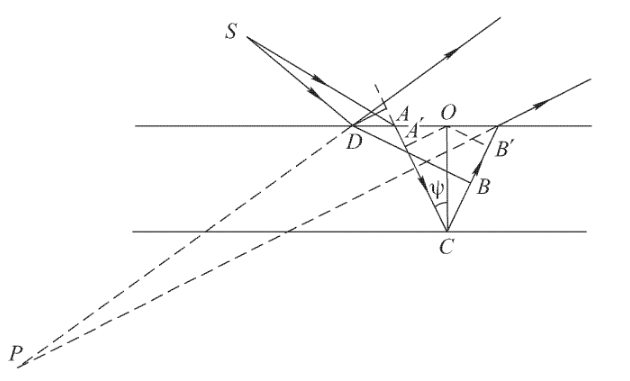
\includegraphics[width=0.3\textwidth]{figures/33_2.png}
    \hspace{5 mm} 
    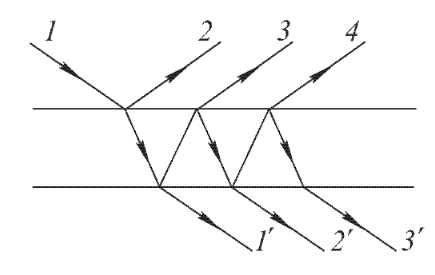
\includegraphics[width=0.2\textwidth]{figures/33_3.png}
    \caption{К интерференции в пленках и пластинках}
    \label{fig:33}
\end{figure}
Интереференция может наблюдаться как в отраженном свете, так и в преломленном, однако проще всего наблюдать интерференцию света на самой пластинке. 
Если рассмотреть потерю в 5\% при отражении, то увидим, что основная интенсивность приходится на лучи $2,\, 3$ и $1'$ (рис. \ref{fig:33}). 




\textbf{Кольца Ньютона}. 
Если прижать линзу к пластинке, то будут интерференционные \textit{колечки Ньютона}. Можно показать, что разность хода будет
\begin{equation*}
    d= \frac{x^2}{2R}, \hspace{10 mm} \Delta = 2 d + \frac{\lambda}{2} = \frac{x^2}{R} + \frac{\lambda}{2},
\end{equation*}
где $R$ -- радиус кривизны линзы, а $x$ -- полярная координата. Светлый кольца будут при $\Delta = m \lambda $, тогда радиум $m$-го светлого кольца:
\begin{equation*}
    x_m^{\text{светл}} = \sqrt{\left(m-\frc{1}{2}\right) \lambda R} = \sqrt{\lambda R/2} \sqrt{2m-1},
    \hspace{5 mm} 
    x_m^{\text{тёмн}} = \sqrt{m \lambda R} = \sqrt{\lambda R/2} \sqrt{2m}.
\end{equation*}